%% =====================================================================
%%  Runcell / NotebookMind -- project report
%%  ACM LaTeX template, single column (manuscript mode)
%%  Compile in Overleaf with pdfLaTeX. Bibliography: BibTeX (references.bib).
%%
%%  Screenshots: put PNG files into  report/figures/  using the file names
%%  given in each \shot{...} below. If a file is missing the document still
%%  compiles and prints a labelled placeholder box in its place.
%% =====================================================================

\documentclass[manuscript]{acmart}

%% ---- Housekeeping for a course submission ---------------------------
\settopmatter{printacmref=false}                    % no ACM reference block
\renewcommand\footnotetextcopyrightpermission[1]{}  % no copyright strip
\pagestyle{plain}
\setcopyright{none}
\acmConference[PIIS SoSe 2026]{Practical Intelligent Interactive Systems}%
  {Sommersemester 2026}{Munich, Germany}

%% ---- Packages -------------------------------------------------------
\usepackage{graphicx}
\usepackage{booktabs}
\usepackage{tikz}
\usetikzlibrary{positioning,arrows.meta,shapes.geometric,fit,backgrounds,calc}

%% Screenshot helper: prints the image if present, else a placeholder box.
\newcommand{\shot}[2]{%
  \IfFileExists{figures/#1}%
    {\includegraphics[width=\linewidth]{figures/#1}}%
    {\fbox{\parbox[c][40mm][c]{\dimexpr\linewidth-2\fboxsep-2\fboxrule\relax}%
      {\centering\ttfamily\footnotesize figures/#1\\[2mm]%
       \normalfont\itshape\footnotesize #2}}}%
}

%% TikZ styles for the diagrams
\tikzset{
  boxy/.style   ={rectangle, rounded corners=2pt, draw=black!55, fill=black!3,
                  align=center, font=\small, inner sep=5pt, minimum height=8mm},
  layer/.style  ={rectangle, rounded corners=3pt, draw=black!25, fill=black!2,
                  inner sep=8pt},
  flow/.style   ={-{Stealth[length=2.4mm]}, draw=black!65},
  dashflow/.style={-{Stealth[length=2.4mm]}, draw=black!45, dashed},
  lbl/.style    ={font=\scriptsize\itshape, midway, fill=white, inner sep=1pt},
  slbl/.style   ={font=\scriptsize\itshape, align=center, inner sep=1pt}
}

\begin{document}

%% =====================================================================
\title{Runcell: A Gamified and Privacy Preserving Learning Layer Inside
JupyterLab}
\subtitle{Turning a course's own notebooks into verified exercises, and class
telemetry into anonymous teaching signal}

\author{Yunes Mahan}
\affiliation{%
  \department{Fakult\"at f\"ur Mathematik, Informatik und Statistik}
  \institution{Ludwig-Maximilians-Universit\"at M\"unchen}
  \city{Munich}
  \country{Germany}}
\email{y.mahan@campus.lmu.de}

%% =====================================================================
\begin{abstract}
Computational notebooks are the default medium for teaching data science, yet
they are pedagogically passive: a student can scroll a finished notebook, run
every cell, watch correct output appear, and finish having practised nothing.
Notebook tooling for education is dominated by assessment infrastructure such
as \texttt{nbgrader}, which marks submissions well but does not change what
happens while the student reads. We present \emph{Runcell}, a JupyterLab~4
extension that turns a course's existing notebooks into an active learning
experience without asking teachers to rewrite their material. Runcell derives
three kinds of exercise from each code cell using a large language model,
verifies answers by executing them on the live Jupyter kernel and comparing
runtime output rather than source text, and layers experience points, an opt in
leaderboard and consent based peer comparison on top. Its instructor dashboard
is built on \emph{anonymous} per cell attempt records, so teachers see which
cells the class fails without being able to attribute a failure to a named
individual. Our contributions are an output equivalence verification loop that
admits any working solution instead of one canonical answer, a privacy
asymmetry in which motivational features are identified and diagnostic features
are anonymous by construction, and a degradation design in which the system
stays usable with no AI key and no backend.
\end{abstract}

%% ---- ACM CCS concepts ----------------------------------------------
\begin{CCSXML}
<ccs2012>
 <concept>
  <concept_id>10010405.10010489.10010492</concept_id>
  <concept_desc>Applied computing~Interactive learning environments</concept_desc>
  <concept_significance>500</concept_significance>
 </concept>
 <concept>
  <concept_id>10010405.10010489.10010491</concept_id>
  <concept_desc>Applied computing~Computer-assisted instruction</concept_desc>
  <concept_significance>300</concept_significance>
 </concept>
 <concept>
  <concept_id>10003120.10003121</concept_id>
  <concept_desc>Human-centered computing~Human computer interaction (HCI)</concept_desc>
  <concept_significance>300</concept_significance>
 </concept>
</ccs2012>
\end{CCSXML}

\ccsdesc[500]{Applied computing~Interactive learning environments}
\ccsdesc[300]{Applied computing~Computer-assisted instruction}
\ccsdesc[300]{Human-centered computing~Human computer interaction (HCI)}

\keywords{computational notebooks, JupyterLab, gamification, programming
education, large language models, learning analytics, privacy by design}

\maketitle

\begin{center}
\small\itshape
Project report for \textnormal{Practical Intelligent Interactive Systems},
Sommersemester 2026.
\end{center}

%% =====================================================================
\section{Introduction}

Jupyter notebooks are the standard delivery format for teaching data analysis,
scientific computing and applied machine learning \cite{kluyver2016jupyter}. A
typical week ships slides and notebooks in which the instructor has already
written the code, already executed it and already saved the output. The intent
is that the student reads the narrative, runs the cells and internalises the
reasoning. The observed behaviour is different: because the notebook arrives
complete, the cheapest path through it is to press Shift and Enter repeatedly,
watch plots appear and reach the last cell in minutes. The student has produced
a perfect artifact and has practised nothing.

This is not hypothetical. Roughly one in four notebooks on GitHub contains no
prose at all, and among academic notebooks most describe what was done without
discussing why or what the result means \cite{rule2018exploration}; a large
fraction do not even execute reproducibly in order
\cite{pimentel2019largescale}. The medium optimises for exploration and for
presenting a finished result, neither of which is optimising for learning.

The learning sciences explain what is missing. Retrieval practice, producing an
answer rather than rereading it, yields substantially better long term
retention than restudying \cite{roediger2006power}; explaining a step to
oneself improves comprehension and transfer \cite{chi1994eliciting}; and
feedback works best when it is immediate, task specific and tells the learner
how to close the gap \cite{hattie2007power}. A pre executed notebook offers
recognition instead of recall, presentation instead of explanation, and no
feedback loop at all, because there is nothing the student can get wrong.

Existing notebook tooling addresses a different problem. \texttt{nbgrader}, the
reference solution, is an assignment and grading pipeline
\cite{blank2019nbgrader}: author a master notebook with hidden tests, release a
stripped student version, collect and autograde. It solves assessment well, but
it does not change the experience of reading course material, and every
exercise must still be written by hand with its own tests.

\medskip
\noindent\textbf{Problem statement.} \emph{How can a course's existing,
unmodified notebooks be turned into an active, feedback rich learning
experience, without requiring the instructor to author exercises by hand, and
without turning the resulting telemetry into a surveillance instrument aimed at
individual students?}

\medskip
Runcell answers that as a JupyterLab~4 extension with two modes, \emph{Learn}
and \emph{Explain}, described in Section~\ref{sec:learn}. Behind both sits a
course backend that tracks progress, ranks students on an opt in leaderboard
and feeds an instructor dashboard built exclusively on anonymous aggregates.

%% =====================================================================
\section{Background and Related Work}
\label{sec:related}

\paragraph{Assessment tooling.}
\texttt{nbgrader} \cite{blank2019nbgrader} defines the state of practice, and
variants such as Otter Grader follow the same batch shape. Two properties
matter for our positioning: feedback is delayed until grading, the opposite of
what the feedback literature recommends \cite{hattie2007power}, and correctness
is defined by instructor written unit tests, so authoring effort scales with
the amount of material. Runcell does not compete on grading; it targets the
reading phase, and derives exercises rather than requiring them to be written.

\paragraph{Gamification in programming education.}
Sailer and Homner \cite{sailer2020gamification} report small but real positive
effects of gamification on cognitive ($g = 0.49$), motivational ($g = 0.36$)
and behavioural ($g = 0.25$) outcomes. Crucially the effect depends on which
elements are used: reward and status mechanics bolted onto unchanged content
perform noticeably worse than designs adding genuine challenge. Self
determination theory explains why \cite{ryan2000selfdetermination}: points and
rankings are controlling extrinsic regulators that can crowd out intrinsic
motivation when they are the only change. We therefore did not gamify reading.
We changed the activity from reading to solving and only then attached points,
and we made the leaderboard opt in, because a ranking a student cannot decline
is exactly the mechanic the literature warns about.

The closest prior systems come from the Learning Technologies group at RWTH
Aachen, who integrate game elements into Jupyter driven by learning analytics
\cite{brocker2022integration,brocker2022gamifying}, logging JupyterLab
interaction events into a Learning Record Store via xAPI and using that stream
as the substrate for game elements. The difference is where the game lives. In
their design the notebook is unchanged and the gamification observes
interaction with it, so a student who runs every cell without thinking still
generates activity; in Runcell the notebook itself is transformed, so points
cannot be earned without producing a correct artifact. We also add a course
model, instructor authoring and an analytics surface.

\paragraph{Exercise types and authoring cost.}
Parsons problems, in which a student reassembles scrambled code fragments, are
the best studied alternative to free code writing. Reviews
\cite{du2020review,ericson2022parsons} report that they reduce working memory
load, in line with cognitive load theory \cite{sweller1988cognitive}, and reach
outcomes comparable to equivalent code writing exercises in less student time;
the caveat is that authoring good problems with plausible distractors is
expensive. Runcell borrows the underlying idea, that a spectrum of scaffolding
between reading code and writing it from nothing is valuable, and derives each
of its three exercise types from the cell the instructor already wrote.

\paragraph{Large language models in computing education.}
Sarsa et al. \cite{sarsa2022automatic} showed that an LLM can generate
programming exercises with sample solutions and test cases at a quality that is
usable but not uniformly reliable, so generated artifacts need verification
before students see them. CodeHelp \cite{liffiton2023codehelp} deployed an LLM
assistant with guardrails preventing it from emitting full solutions, and found
it complemented rather than replaced human help. Denny et al.
\cite{denny2024computing} set out the broader framing: because models solve
introductory assignments outright, assessment must move towards process,
comprehension and explanation. Runcell therefore treats the AI as a content
generator and tutor rather than a gatekeeper, and never trusts its answer key.

\paragraph{Learning analytics and its ethics.}
Instructor dashboards showing per student progress are standard, and they are
also the part of learning analytics that draws the most serious objections.
Slade and Prinsloo \cite{slade2013learning} catalogue the dilemmas: data
ownership, what informed consent means when participation is compulsory, and
the tension between care and surveillance. An early iteration of our system had
a per student drill down showing an individual's attempts cell by cell; it was
removed after a formative review whose strongest message was that instructors
should see \emph{where the class fails} without seeing \emph{who failed}. To
our knowledge the resulting asymmetry, in which the motivational subsystem is
identified and consensual while the diagnostic subsystem is structurally
anonymous at the storage layer, is absent from the systems surveyed above.

%% =====================================================================
\section{Design Goals}
\label{sec:goals}

The analysis above, plus a formative review of an early prototype, produced six
goals we treat as requirements and justify later decisions against.

\begin{description}
\item[G1. Zero authoring cost.] A teacher publishes an ordinary notebook and
exercises exist for it immediately, while keeping the ability to override any
generated exercise by hand.
\item[G2. Correctness by execution.] Any code producing the required result
must be accepted. There is more than one correct way to write almost every
cell, and rejecting a working solution for not matching a reference string is
both wrong and demoralising.
\item[G3. Immediate, task level feedback.] Following \cite{hattie2007power},
the student learns within seconds whether they are right, and when wrong
receives a graduated nudge rather than the answer.
\item[G4. Motivation without coercion.] Points are on by default because they
attach to genuine challenge; social comparison is opt in, because a mandatory
ranking is the mechanic that
\cite{sailer2020gamification,ryan2000selfdetermination} call counterproductive.
\item[G5. Diagnostic value without surveillance.] The instructor gets class
level failure signal, and the storage layer must make individual attribution
impossible rather than merely hidden.
\item[G6. Graceful degradation.] The system stays useful with no AI key, no
backend and no course at all.
\end{description}

%% =====================================================================
\section{System Architecture}
\label{sec:arch}

Runcell is a JupyterLab~4 extension in three layers (Figure~\ref{fig:arch}).
Building an extension rather than a separate web application follows from G2:
verification needs a real Python kernel with the course libraries installed,
and inside JupyterLab that kernel already exists. A standalone application
would have had to provision and sandbox its own execution environment.

\begin{figure}[t]
\centering
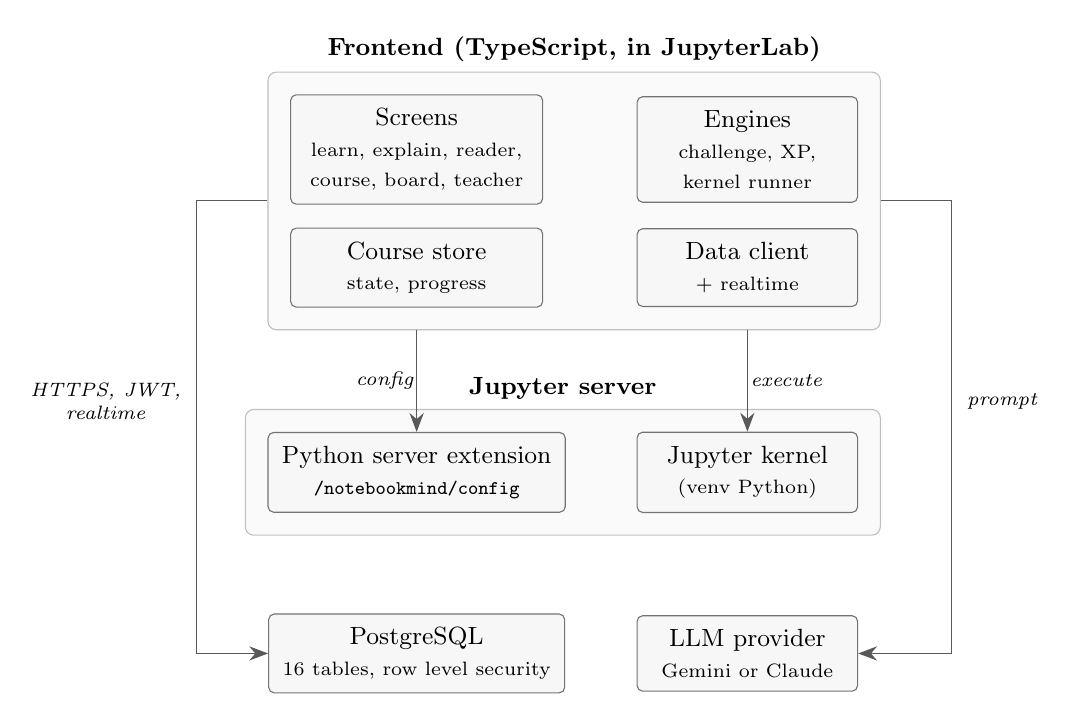
\begin{tikzpicture}[x=1cm,y=1cm]

%% ---- Frontend tier -------------------------------------------------
\node[boxy, minimum width=32mm] (screens) at (0,0) {Screens\\\scriptsize learn,
explain, reader,\\\scriptsize course, board, teacher};
\node[boxy, minimum width=28mm] (engines) at (4.2,0) {Engines\\
\scriptsize challenge, XP,\\\scriptsize kernel runner};
\node[boxy, minimum width=32mm] (store) at (0,-1.5) {Course store\\
\scriptsize state, progress};
\node[boxy, minimum width=28mm] (dbclient) at (4.2,-1.5)
{Data client\\\scriptsize + realtime};

\begin{scope}[on background layer]
\node[layer, fit=(screens)(engines)(store)(dbclient),
      label={[font=\small\bfseries]above:Frontend (TypeScript, in JupyterLab)}]
      (front) {};
\end{scope}

%% ---- Jupyter server tier -------------------------------------------
\node[boxy, minimum width=32mm] (server) at (0,-4.1)
{Python server extension\\\scriptsize \texttt{/notebookmind/config}};
\node[boxy, minimum width=28mm] (kernel) at (4.2,-4.1)
{Jupyter kernel\\\scriptsize (venv Python)};

\begin{scope}[on background layer]
\node[layer, fit=(server)(kernel),
      label={[font=\small\bfseries]above:Jupyter server}] (mid) {};
\end{scope}

%% ---- External services ---------------------------------------------
\node[boxy, minimum width=34mm] (pg) at (0,-6.4)
{PostgreSQL\\\scriptsize 16 tables, row level security};
\node[boxy, minimum width=28mm] (llm) at (4.2,-6.4)
{LLM provider\\\scriptsize Gemini or Claude};

%% ---- Wiring (orthogonal, no box is crossed) ------------------------
\draw[flow] (front.south -| server) --
      node[lbl,left]{config} (server.north);
\draw[flow] (front.south -| kernel) --
      node[lbl,right]{execute} (kernel.north);
\draw[flow] (front.west) -- ++(-0.9,0) |- (pg.west);
\draw[flow] (front.east) -- ++(0.9,0) |- (llm.east);
\node[slbl, anchor=east] at (-2.95,-3.2) {HTTPS, JWT,\\realtime};
\node[slbl, anchor=west] at (6.95,-3.2) {prompt};
\end{tikzpicture}
\caption{Three layer architecture. The frontend talks to three independent
services: the kernel for verification, the LLM for generation, PostgreSQL for
state. Any can be absent without taking the others down.}
\label{fig:arch}
\end{figure}

The frontend is about 16{,}000 lines of TypeScript across 51 modules,
registering one JupyterLab plugin that boots a login overlay, fetches
configuration from the server extension and mounts a full screen widget into
the shell. Screens are plain DOM modules with a shared design system rather
than a component framework, since adding React to an extension bundle
materially increases build complexity and size for a project whose
interactivity is mostly local to individual cards. Code editing uses
CodeMirror~6 with the Python mode, the editor JupyterLab itself uses.

The Python side is thin: a server extension exposing one endpoint that reads a
local \texttt{.env} and returns the LLM key and the database credentials. It
exists because a browser extension has no filesystem access, so without it
every user would have to paste API keys into the interface.

State lives in a PostgreSQL database on Supabase, accessed directly from the
browser over HTTPS with a JSON Web Token issued at sign in. There is no bespoke
application server: a REST API in Python would have meant reimplementing
authentication, session refresh, authorization and websocket fan out. Instead
authorization is expressed once as row level security policies in the database,
enforced for every query regardless of client, and live updates arrive over
Supabase Realtime, which streams the logical replication feed to subscribers
while applying the same policies. The security perimeter is the database, not
the client. The schema is sixteen tables and eight stored procedures over
twenty one ordered migrations.

%% =====================================================================
\section{The Learning Experience}
\label{sec:learn}

\subsection{Learn mode: three exercise types}

In Learn mode the notebook is not shown. The student is walked through it one
code cell at a time, and each cell is presented as one of three exercise types
(Table~\ref{tab:types}).

\begin{table}[t]
\caption{Exercise types and how answers are verified. Free text prediction was
implemented and then disabled, because grading it requires trusting the model.}
\label{tab:types}
\centering\small
\begin{tabular}{@{}p{26mm}p{56mm}p{56mm}@{}}
\toprule
\textbf{Type} & \textbf{Student produces} & \textbf{Verified by} \\
\midrule
Fix the bug & A corrected version of code containing exactly one planted
defect & Kernel execution, output compared to the original cell \\
\addlinespace
Write the cell & The whole cell from scratch, given a written brief & Kernel
execution, output compared to the original cell \\
\addlinespace
Comprehension & One of four options describing what the already executed cell
does & Match against the generated answer key \\
\bottomrule
\end{tabular}
\end{table}

The three types form a scaffolding ladder in the sense of the Parsons
literature \cite{ericson2022parsons}. Comprehension imposes the least
generative load, since code and output are both visible and the task is to
reason about effect. Fix the bug imposes more: the student must hold a correct
mental model of the cell and locate where the code diverges from it. Write the
cell imposes the most, since the editor starts empty and the student
reconstructs the computation from a brief. That is retrieval practice in the
strict sense \cite{roediger2006power}, and it is the fallback type.

Each exercise carries a difficulty label from easy to impossible, which sets
the reward at 2, 4, 6 or 10 experience points; finishing a notebook is worth
30. The values are not empirically tuned. They exist to make harder work
visibly more valuable, the property that matters for the challenge oriented
gamification \cite{sailer2020gamification} finds effective.

\begin{figure}[t]
\centering
\shot{learn-mode.png}{Screenshot: Learn mode. Capture a fix the bug exercise
with the brief at the top, the code editor, and the hint box open.}
\caption{Learn mode. The brief names the actual variables the cell touches, and
Run and check executes the answer on the live kernel.}
\label{fig:learn}
\end{figure}

\subsection{Generation and verification}

Figure~\ref{fig:pipeline} shows the loop. Before the session starts, Runcell
executes the original notebook cell by cell on a fresh kernel and records the
normalised output of every cell. That is the reference. Generation then sends
the cell source to the LLM with a schema constrained prompt naming the three
permitted types, forbidding free text answers, and demanding that the brief
reference the real objects in the cell rather than generic filler.

The reply is never used as returned. It passes through a coercion function that
repairs or rejects it: an unknown type is replaced, a fix the bug exercise that
arrived without buggy code is rejected, a multiple choice exercise with fewer
than two options is rejected, and a write the cell exercise that arrived pre
populated is emptied. Any rejection falls through to a deterministic exercise
built from the source alone. This is our operational answer to the reliability
caveat in \cite{sarsa2022automatic}: we constrain the output shape, validate it
mechanically, and make the failure mode a safe exercise rather than a broken
one.

Verification is the part we consider strongest. When the student presses Run
and check, their code executes on the same kernel that produced the reference,
and the run is accepted if and only if it did not raise and its normalised
output equals the reference. Normalisation collapses line endings, trailing
whitespace and repeated blank lines, so cosmetic variation does not fail a
correct answer. Because the comparison is on runtime output rather than source
text, a student who writes a comprehension where the instructor wrote a loop is
accepted. This satisfies G2 and it is what makes generated exercises safe: the
model proposes a task, the kernel decides the outcome.

\begin{figure}[t]
\centering
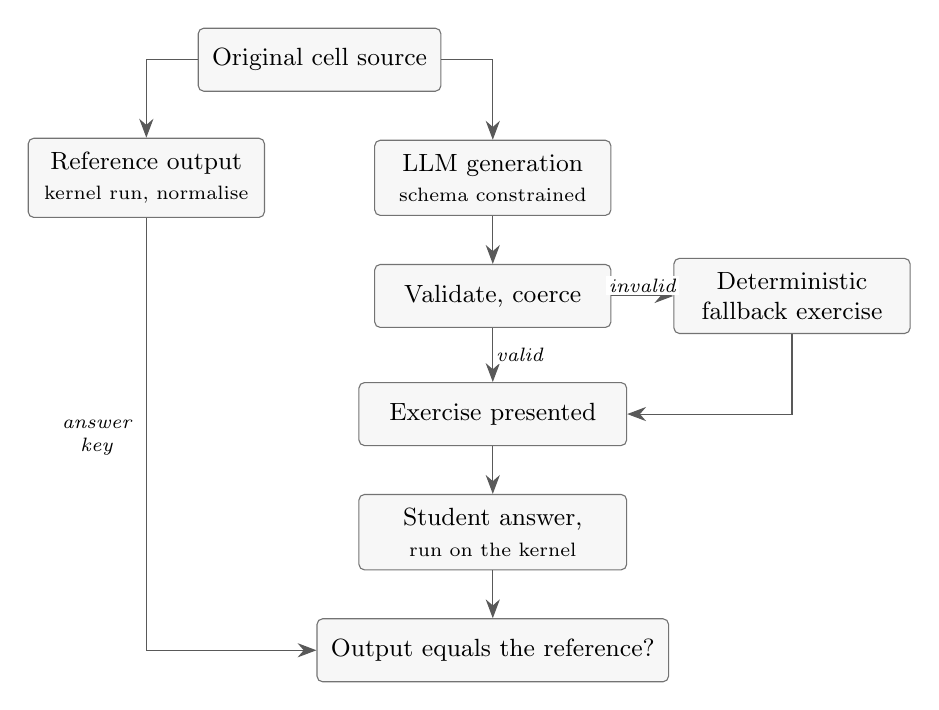
\begin{tikzpicture}[x=1cm,y=1cm]
%% left column: the reference; right columns: generation
\node[boxy, minimum width=30mm] (cell)     at (0,0)      {Original cell source};
\node[boxy, minimum width=30mm] (ref)      at (-2.2,-1.5){Reference output\\
      \scriptsize kernel run, normalise};
\node[boxy, minimum width=30mm] (gen)      at (2.2,-1.5) {LLM generation\\
      \scriptsize schema constrained};
\node[boxy, minimum width=30mm] (coerce)   at (2.2,-3.0) {Validate, coerce};
\node[boxy, minimum width=30mm] (fallback) at (6.0,-3.0) {Deterministic\\
      fallback exercise};
\node[boxy, minimum width=34mm] (task)     at (2.2,-4.5) {Exercise presented};
\node[boxy, minimum width=34mm] (answer)   at (2.2,-6.0) {Student answer,\\
      \scriptsize run on the kernel};
\node[boxy, minimum width=44mm] (cmp)      at (2.2,-7.5) {Output equals the
      reference?};

\draw[flow] (cell.west)  -| (ref.north);
\draw[flow] (cell.east)  -| (gen.north);
\draw[flow] (gen)    -- (coerce);
\draw[flow] (coerce) -- node[lbl,above]{invalid} (fallback);
\draw[flow] (coerce) -- node[lbl,right]{valid} (task);
\draw[flow] (fallback.south) |- (task.east);
\draw[flow] (task)   -- (answer);
\draw[flow] (answer) -- (cmp);
\draw[flow] (ref.south) -- (ref.south |- cmp.west) -- (cmp.west);
\node[slbl, anchor=east] at (-2.35,-4.8) {answer\\key};
\end{tikzpicture}
\caption{Generation and verification. The model only proposes the task; the
answer key is the output the instructor's own cell produced, so any working
solution is accepted and a badly generated exercise degrades to a safe
fallback. A failed comparison returns the student to the exercise with the next
hint unlocked.}
\label{fig:pipeline}
\end{figure}

\subsection{The help ladder and adaptive difficulty}

When a run fails, the student is told whether the cell raised an error or
produced the wrong result, and the raw output is shown. Hints are revealed one
at a time and only on request. A Reveal the answer control is hidden initially
and appears once the learner has either taken a hint or had a run fail, so it
is never the first thing offered. Taking a hint or failing a run clears the
first try flag, which is recorded but does not reduce the experience points
awarded for eventually solving the cell; only revealing the answer forfeits
them. This is the graduated feedback of G3: the student is never stuck, never
handed the answer without asking, and never punished twice for asking. A
difficulty bias of easier, normal or harder is injected into the generation
prompt, and on the harder setting a failed run stops offering the reveal at
all, so a student who asked for a harder session does not get an early escape
hatch. It is the one place where the learner regulates their own challenge
level, the autonomy component of motivation in self determination theory
\cite{ryan2000selfdetermination}.

\subsection{Explain mode and supporting surfaces}

Learn mode is demanding, and it is the wrong mode for a first encounter with
unfamiliar material. Explain mode is the reading counterpart: the notebook
becomes a sequence of cards, one per cell, each showing the code, its output,
and a tabbed context panel with three sources of knowledge. The first is an AI
explanation of what the cell does, plus a tutor chat scoped to that one cell;
the second is the instructor's note with the week's slide embedded inline; the
third is the peer comment thread. Embedding the slide
beside the cell rather than behind a separate materials button came from
formative feedback, since students had been reading code in one place and
slides in another.

On wide screens each card is flanked by margin columns for private sticky
notes. These are the one piece of content in the system that is strictly
private: they persist to the student's own account, survive reload, and are
readable by nobody else, not classmates and not the instructor. The intent is
to give the student a place to record the moment they understood something, the
self explanation behaviour \cite{chi1994eliciting} shows to be beneficial, and
to make that place safe enough that they use it.

Around the two modes sit a course home with a week timeline, a slide and paper
reader with quizzes and flashcards whose review date is pushed out by how the
learner rated the card, a course map of the dependency structure between
topics, and a leaderboard with a friends screen. One surface defines the
system's floor: Bring your own notebook lets a user upload an arbitrary
\texttt{.ipynb} file and learn it with no course and no instructor, keeping it
on the device in IndexedDB rather than in their account, so the file itself is
never transmitted.

\begin{figure}[t]
\centering
\shot{explain-mode.png}{Screenshot: Explain mode. Capture one cell card with
the context tabs visible, an embedded slide, and at least one yellow margin
note.}
\caption{Explain mode. Every cell carries an AI explanation and tutor chat, the
instructor's note with the week's slide inline, the peer comment thread, and
private margin notes.}
\label{fig:explain}
\end{figure}

%% =====================================================================
\section{The Teaching Side}
\label{sec:teach}

An instructor creates a course, receives an invite code, and publishes weeks of
notebooks and slides that can be locked or unlocked to control pacing. Per cell
notes are authored in Markdown, and generated exercises can be overridden with
hand written tasks, which is how G1 preserves instructor control: generation is
the default, not the only option.

\subsection{Analytics without attribution}

The dashboard answers three questions. Which cells does the class fail? Which
topics are weak? Is the class progressing? It answers them from two aggregate
stored procedures and one anonymous table.

Per cell difficulty comes from the \texttt{cell\_attempts} table, which has no
user column at all: a row records the notebook, the cell index, the course,
whether the attempt succeeded and which attempt number it was. The instructor
sees, per cell, a struggle score computed as one minus the first try rate,
ordered worst first. This is the mechanism behind G5, and the important
property is that it is enforced by the shape of the data rather than by the
interface: even a database administrator running arbitrary SQL cannot recover
who failed a given cell.

Per topic understanding comes from \texttt{notebook\_submissions}, which does
carry a user reference, aggregated by notebook title into a stacked bar of
understood versus struggled proportions; the roster shows enrolled students
ranked by course experience points, with their notebooks completed and their
overall first try rate. The boundary is therefore drawn at the cell, not at the
student: an instructor can see that someone is finding the course hard, which
is what lets them offer help, but cannot see \emph{which cell} any named
student failed, because that is the record carrying no identity. The dashboard
labels its own header \emph{Aggregates only}.

The dashboard also writes an algorithmic summary of the aggregates
continuously, without any model call; a separate button sends the same
aggregates to the LLM for a prose report. The AI report never runs
automatically, because live data changes would otherwise trigger a paid model
call on every submission, and reports are cached with a signature of the data
they came from, so when the numbers move the report is marked stale rather than
silently misleading the instructor. Six tables are published to the realtime
feed, so a student joining, submitting or commenting repaints the dashboard and
the affected Explain mode threads without a reload.

\begin{figure}[t]
\centering
\shot{teacher-dashboard.png}{Screenshot: teacher dashboard Overview, showing
the per topic understanding chart and the insights card.}
\caption{Instructor dashboard. Per topic first try mastery, weakest first, with
counts of students and cells but no names attached to any failure. Below it the
algorithmic summary updates continuously, while the AI report stays behind an
explicit button.}
\label{fig:teacher}
\end{figure}

%% =====================================================================
\section{Privacy and Security Model}
\label{sec:privacy}

Table~\ref{tab:visibility} states who can see what. The pattern is an
asymmetry: everything that motivates is identified and consensual, everything
that diagnoses is anonymous.

\begin{table}[t]
\caption{Visibility matrix. Failure data is anonymous at the storage layer;
social data requires explicit and revocable consent.}
\label{tab:visibility}
\centering\small
\begin{tabular}{@{}p{44mm}p{26mm}p{26mm}p{30mm}@{}}
\toprule
\textbf{Data} & \textbf{Owner} & \textbf{Peers} & \textbf{Instructor} \\
\midrule
Private cell notes      & yes & no & no \\
Per cell attempts       & n/a & no & aggregate only \\
Notebook submissions    & yes & no & yes \\
Experience points       & yes & if opted in & yes \\
Leaderboard rank        & yes & if opted in & yes \\
Friend statistics       & yes & if mutual & no \\
Peer comments           & yes & yes & yes \\
\bottomrule
\end{tabular}
\end{table}

\textbf{Row level security everywhere.} Every table has policies enabled and
explicit grants. The client holds only an anonymous key plus the user's own
token, so the key can be published safely and authorization is decided by
PostgreSQL for every query. Where a query legitimately needs to read across
users, such as ranking a leaderboard, it is a stored procedure that runs with
elevated rights but first checks that the caller is enrolled. That pattern also
resolved a policy recursion cycle in which the courses policy consulted
enrolments and the enrolments policy consulted courses.

\textbf{Opt in leaderboards, scoped per course.} A student appears only if they
set the opt in flag, and rankings use points earned in that course rather than
a lifetime total, so work in one course does not inflate standing in another.
This required tagging every point event with its course, a schema change made
specifically to fix the leak.

\textbf{Mutual consent for peer comparison.} Friend links are directional. One
direction means "I have chosen to share my statistics with you" and reveals
nothing in return; statistics become visible only when both directions exist,
and either side can withdraw at any moment. A stored procedure also lets a user
delete their own account, which cascades every row they own.

%% =====================================================================
\section{Implementation and Validation}

\subsection{Degradation ladder}

G6 is an explicit ladder, each rung a supported state rather than an error.
With \emph{no AI key}, every exercise becomes the deterministic write the cell
type and explanations fall back to written defaults; courses, verification,
points, leaderboards and analytics are unaffected, because none of them depend
on the model. With \emph{no backend}, the extension runs locally: uploads go to
IndexedDB and progress is session scoped, but the learning loop is intact
because verification needs only the kernel. With \emph{no kernel}, verification
degrades to comparing the student's source against the reference source, the
only rung where G2 is sacrificed.

A verification loop built on kernel execution also inherits the fragility of
environment management. For a period during development no cell would execute,
because the kernel specification named an interpreter resolved from the system
path rather than the project's virtual environment. The setup scripts now bind
the kernel to that environment by absolute path.

\subsection{Validation}

Backend correctness is checked by an automated suite that runs against the live
database using the same client library as the application, covering 23 sections
and 76 assertions and exiting non zero on failure. It spans authentication,
profiles, course creation and invite enrolment, the instructor dashboard
aggregates, points and the opt in leaderboard, per cell attempts, notebook and
comment synchronisation, the generated exercise cache, the friend life cycle
from request through mutual sharing to withdrawal, account deletion, a live
realtime event and a live model completion. On the run taken for this report 72
assertions passed, none failed and four skipped: the on device upload, which is
IndexedDB and therefore verifiable only in a browser; the destructive delete
round trip and the realtime publication check, both of which need a direct
Postgres connection string rather than the public key; and sign up, which the
shared project throttles by an email rate limit. The realtime delivery check is
timing sensitive and times out against a cold socket on the free tier, so it
needs a warm connection to pass.

Two properties matter. The suite exercises the real deployment rather than
mocks, so a row level security policy that is wrong in production fails the
test; and it asserts negative cases, such as a non instructor being refused the
dashboard call and a second user being unable to read a student's private
notes, which is the only way to test a privacy claim.

%% =====================================================================
\section{Discussion}

\subsection{What is new}

First, \emph{output equivalence verification for generated exercises}. Prior
work showed that models can generate programming exercises but need review
before use \cite{sarsa2022automatic}, and that automated grading works when an
instructor writes the tests \cite{blank2019nbgrader}. Runcell combines them by
taking the answer key from the instructor's own already executed cell, so
authoring cost drops to zero while the acceptance criterion becomes more
permissive, not less.

Second, the \emph{privacy asymmetry} of Section~\ref{sec:privacy}. Learning
analytics dashboards conventionally present per student detail, and the ethical
literature has argued at length against exactly that \cite{slade2013learning}.
Runcell splits the telemetry: data that motivates is identified and opt in,
data that diagnoses is anonymous by construction. Because the anonymity lives
in the schema rather than in an access control rule, it survives changes to the
interface and to policy.

Third, the \emph{degradation ladder}: a system whose learning loop stops when a
paid API key expires cannot be given to a class. Each of these carries an
accepted cost. Being an extension buys a kernel with the course libraries but
requires an installation step; having no application server keeps authorization
in one place but ties the system to one platform; and anonymous attempt records
buy diagnostic honesty at the price of individual follow up.

\subsection{Limitations and future work}

The most significant limitation is that we have no controlled evaluation of
learning outcomes. The system was validated technically and shaped by formative
feedback, but no study compares students using Runcell against students reading
the same notebooks conventionally, so every pedagogical claim here rests on the
cited literature and on the design following from it rather than on measured
effect.

Output equivalence has a real failure mode: cells whose result is a plot, a
random sample or a wall clock timing do not produce stable comparable text, and
although the system captures images separately it does not compare them.
Generation quality varies with the model, and the validation layer turns poor
generations into safe fallbacks rather than good exercises, so a weak model
produces a monotonous session of write the cell tasks. Finally, the deployment
depends on one hosted backend platform and has been exercised at the scale of a
seeded course rather than a live cohort.

The clearest next step is a controlled study measuring retention and transfer
against conventional notebook reading, with the anonymous attempt data as the
natural instrument since it is already aggregate and needs no further consent.
Structural comparison of plot outputs would extend verification to
visualisation heavy material, and an instructor approval queue for generated
exercises would let a course lift quality where it matters.

%% =====================================================================
\section{Conclusion}

Runcell addresses a widespread failure of computational notebooks as a teaching
medium: the finished notebook invites recognition where learning requires
retrieval. Rather than asking instructors to rewrite their material as
exercises, it derives exercises from what they already have, and rather than
trusting a language model to grade, it lets the Python kernel decide by
comparing what the student's code does against what the instructor's cell did.
Around that loop sit a course model, a progression system whose social features
are opt in and revocable, and an instructor dashboard whose per cell failure
signal is anonymous in the schema rather than in the interface. Its pedagogical
effect remains to be measured.

%% =====================================================================
\phantomsection
\section*{Contributions}

Runcell was built by Yunes Mahan and Johannes Specht as a two person project,
with the work split evenly. We met weekly to plan the next increment, settle
the design decisions justified in this report, and divide that week's tasks
into two comparable halves. Neither of us owned a subsystem outright: both of
us worked across the TypeScript frontend, the Postgres schema and its row level
security policies, and the test suite, and each week's output was reviewed by
the other before it was merged. This report is written and submitted
individually, as the course requires.

%% =====================================================================
\phantomsection
\section*{Availability}

Source code, database migrations, setup scripts and the automated test suite
are available at

\begin{center}
\url{https://github.com/yunes-mahan/NotebookMind}
\end{center}

\noindent
The repository README documents system requirements, a one command setup for
Windows, macOS and Linux, and disposable accounts for a seeded demonstration
course.

%% =====================================================================
\bibliographystyle{ACM-Reference-Format}
\bibliography{references}

\end{document}
